\documentclass{beamer}

\usetheme{Goettingen}

\usecolortheme{rose}

\setbeamercovered{transparent}

\usepackage[english]{babel}
\usepackage[T1]{fontenc}
\usepackage[utf8]{inputenc}
\usepackage{url}

\usepackage{listings}
\usepackage{translator}
\usepackage{enumitem}

\newenvironment{program}{\begin{beamercolorbox}[rounded=true,shadow=true]{block body}\vspace{-4mm}}{\vspace{-2mm}\end{beamercolorbox}}

\setbeamercolor{fvystup}{fg=white,bg=black}
\newenvironment{vystup}{\begin{beamercolorbox}[rounded=true,shadow=true]{fvystup}}{\end{beamercolorbox}}

\newenvironment{poznamka}{\begin{beamercolorbox}[rounded=true,shadow=false]{block body}}{\end{beamercolorbox}}

\setbeamertemplate{section in toc}[sections numbered]

\author{Alžbeta Žiarovská}
\institute{
	Faculty of Informatics and Information Technologies\\
	Slovak Technical University in Bratislava}

\subtitle{\vspace{3mm} Engineering Methods 2023/2024}

\title{Comparative Analysis of the Efficiency of Techniques for Detecting Misinformation in Healthcare Data
}

%ULOHA - zmenit na datum odozvdania
\date{\footnotesize \today}




\begin{document}

\begin{frame}[fragile=singleslide]
\titlepage
\end{frame}


\begin{frame}[fragile=singleslide]\frametitle{Table of Contents}
\tableofcontents
\end{frame}

\section{Motivation and problem}

\begin{frame}[fragile=singleslide]\frametitle{Motivation and problem}
\begin{itemize}[label=$\bullet$]
\item Motivation
	\begin{itemize}[label=$\bullet$]
	\item Personal interest in misinformation
	\item Learning about machine learning techniques
	\end{itemize}
\item Problem
\begin{itemize}[label=$\bullet$]
	\item Perception of information found on the Internet
	\item Everyday use for information retrieval
	\end{itemize}
\end{itemize}
\end{frame}

\section{Related Work}

\begin{frame}[fragile=singleslide]\frametitle{Related Work}
\begin{itemize}[label=$\bullet$]
\item Misinformation
	\begin{itemize}[label=$\bullet$]
	\item Misinformation vs. disinformation
	\item Medical misinformation
	\end{itemize}
\item Machine learning techniques used for information retrieval
	\begin{itemize}[label=$\bullet$]
	\item Naive Bayes
	\item Support Vector Machine
	\end{itemize}
\end{itemize}
\end{frame}



\section{Methodology}

\begin{frame}[fragile=singleslide]\frametitle{Methodology}
\begin{itemize}[label=$\bullet$]
\item Getting general knowledge of the topic
\item Introducing the term misinformation 
\item Introducing Naive Bayes and Support Vector Machine
\item Summarizing and comparing the results found in various sources
\end{itemize}
\end{frame}

\section{Analysis and Results}

\begin{frame}[fragile=singleslide]\frametitle{Analysis and Results}
\begin{table}[H]
\centering
\begin{tabular}{||c c||} 
 \hline
Naïve Bayes & Support Vector Machine\\ [0.5ex] 
 \hline\hline
 $88.37\%$ & $84\%$  \\
 \hline
 $98.71\%$ & $94.17\%$  \\
 \hline
 $85.85\%$ & $90.95\%$  \\
 \hline
 $84.06\%$ & $95.05\%$  \\ [1ex]
 \hline
\end{tabular}
\caption{\centering Accuracy of machine learning techniques in misinformation detection according to various researches}
\label{table:results}
\end{table}
\end{frame}

\begin{frame}[fragile=singleslide]\frametitle{Analysis and Results}
\begin{figure}
\centering
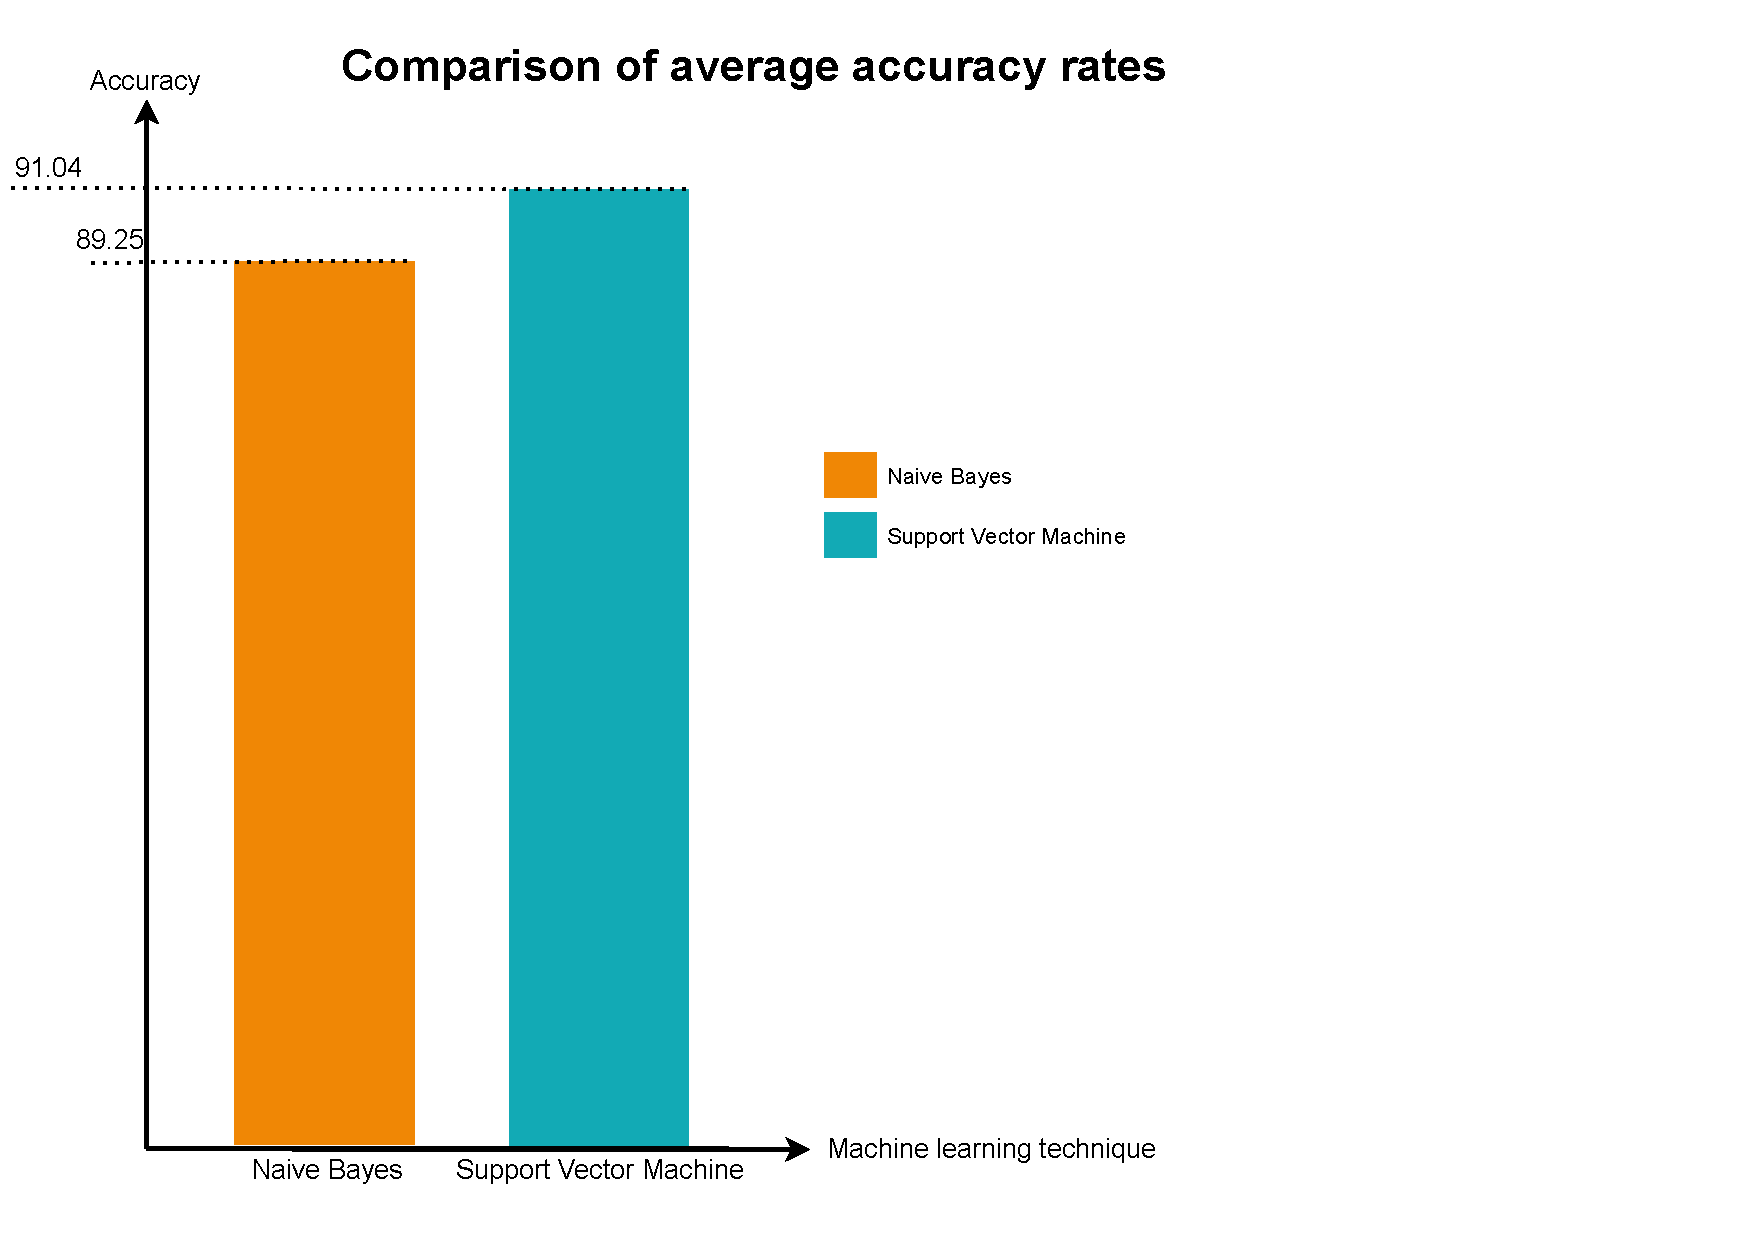
\includegraphics[scale=.35]{average_accuracy.pdf}
\end{figure}
\end{frame}

\section{My Contribution}

\begin{frame}[fragile=singleslide]\frametitle{My Contribution}
\begin{itemize}[label=$\bullet$]
\item Relevant data extraction
\item Efficient differentiation between false and true information
\end{itemize}
\end{frame}

\end{document}




Text za príkazom \end{document} LaTeX ignoruje, takže tu môžete odkladať veci (aj celé slajdy), ktoré nechcete vymazať, lebo ich ešte možno budete potrebovať, avšak ich v danom momente nechcete mať v slajdoch.

\section*{Pomocník}
% hviezdička zabezpečí, aby sa táto časť neocitla v prehľade prezentácie - každá prezentácia má zhodnotenie a prehľad by sa tým zbytočne zahlcoval

\begin{frame}[fragile=singleslide]\frametitle{My Contribution}
\begin{itemize}
\item Každá prezentácia musí byť nejako uzavretá
\item Ale vždy je čo robiť ďalej\ldots{}
\end{itemize}
{\tiny Nejaká poznámka k obrázku, možno zdroj\ldots}
\end{frame}

\begin{frame}[fragile=singleslide]\frametitle{Misinformation in Healthcare}
\begin{itemize}
\item Na zvýraznenie syntaxe stačí použiť balík listings so správne nastaveným programovacím jazykom
\begin{lstlisting}
int na_druhu(int i) {
   return i * i;
}

int main() {
   printf("%d", na_druhu(118));
   return 0;
}
\end{lstlisting}

\item Jazyk C++ je ešte zaujímavejší: je multiparadigmový\footcite{\url{J. O. Coplien. Multi-Paradigm Design for C++. Addison-Wesley, 1998.}}
\end{itemize}
\begin{poznamka}
Text možno uviesť v rámiku
\end{poznamka}

\begin{itemize}
\item Program

\begin{program}
\begin{lstlisting}
void main() {
   printf("%d", na_druhu(118));
}

void na_druhu(int i) {
   return i * i;
}
\end{lstlisting}
\end{program}

\item Výstup
\begin{vystup}
\begin{lstlisting}
13924
\end{lstlisting}
\end{vystup}

\end{itemize}
\end{frame}
